\documentclass[runningheads,a4paper]{article}

\usepackage[utf8]{inputenc}

\setcounter{tocdepth}{3}

\usepackage[english]{babel} 
\usepackage{graphicx}
\usepackage{grffile}
\usepackage{float}
\usepackage{multicol}
\usepackage{url}
\usepackage{array}
\usepackage{wrapfig}
 \usepackage{multirow}
\usepackage{tabu}
\usepackage{amssymb}% http://ctan.org/pkg/amssymb
\usepackage{pifont}% http://ctan.org/pkg/pifont
\usepackage[font=small,labelfont=bf]{caption}

\newcommand{\cmark}{\ding{51}}%
\newcommand{\xmark}{\ding{55}}%

\usepackage{titling}
\usepackage[hidelinks]{hyperref}
\setcounter{secnumdepth}{5}
%Margins
\usepackage[
margin=2cm,
includefoot
]{geometry}


\graphicspath{{/}}

%Headers and Footers
\usepackage{fancyhdr}
\pagestyle{fancy}
\fancyhead{}
\fancyfoot{}
\fancyfoot[R]{\thepage}
\renewcommand{\headrulewidth}{0pt}
\renewcommand{\footrulewidth}{0pt}
\setlength\parindent{24pt}
\begin{document}
	
%Title Page
\begin{titlepage}
	\begin{center}
		
\includegraphics[width=10cm]{UP_Logo.PNG}  \\
		[1cm]
		\line(1,0){300} \\
		[0.3cm]
		\textsc{\Large
			Benchmarking Service\\
			Software Requirements Specification\\
			\hfill
			%University of Pretoria
		}\\
		[0.1cm]
		\line(1,0){300} \\
		[0.7cm]
		\textsc{\Large
			ProCoders
		} \\
	\end{center}
	
	\begin{center}
		\begin{centre}
			\textsc{\large\\
				Bongani Tshela - 14134790\\ 
			}
		
				\textsc{\large\\
					Harris Leshaba - 15312144\\ 
				}
			\textsc{\large\\
				Joseph Letsoalo - 15043844\\ 
			}
			
			\textsc{\large\\
				Minal Pramlall - 13288157\\ 
			}
			

            

		\end{centre}
		
		
		
	\end{center}
\end{titlepage}
%\maketitle%%%%%%%%%%%%%%%%%%%%%%%%%%%%%%%%%%%%%%%%%%%%%%%%%%%%%%%%%%%%%%%%%%%%

\begingroup

\tableofcontents
\addcontentsline{toc}{section}{Table Of Contents}
\endgroup
\newpage

%-------------------------First section---------------------
\section{Introduction}
\subsection{Purpose}
	This document aims to unambiguosly define the requirements of the microbenchmarking web service.
	The document describes the uses of the product including objectives and goals.
	This document is intended for the development team, to enable all members of the team to have the
	same understanding of what should be done. The client can also use the document to verify whether the
	development team understood the needs and goals of the user, partaining to the use of the service.
\subsection{Scope}
	{\bf Product Name: ProBenchmarking}\newline
	Probenchmarking is an online microbenchmarking service that enable users to benchmark thier algorithms
	on different platforms. The users can measure how their algorithms use resouces of the system. 
	They can measure how the algorithms uses a variety of system performance attributes such as CPU time, elapsed time,
	memory usage, power consumption and heat generation.

%-------------------------2nd Section---------------------
\section{Overall Description}
    \begin{flushleft}
	The Benchmarking service will be to provide users with the capability of testing viability between algorithms with graphical data backed by performed tests. Programmers are taught multiple ways to complete a task, and with a benchmarking tool at their disposal, they will be able to make informed decisions with which is the best algorithm to use among the ones that they have considered. 
	\end{flushleft}
	\newline
	\begin{flushleft}
    The service will make use of microkernels, a super-lightweight operating system that will handle user requests and provide results. The system will be run off a cloud infrastructure service such as Google Cloud Compute Engine, to ensure the service is completely online, and thus completely accessible from anywhere with an internet connection.
    \end{flushleft}
    \newline
    \begin{flushleft}	
	The user will communicate with the system through a website interface, they can submit multiple algorithms to benchmark and multiple datasets for them to be tested against. The system will benchmark all of these concurrently and provide the user with graphs and other visual output on the results. \newline
	
	The system will be released into the open-source domain upon completion (Per request of the client). \newline
    \end{flushleft}
	\subsection{Product Perspective}
		A benchmarking service is not easily accessible so this system will be able to provide for that need. Team ProCoder will undertake the development of this service, and provide a reliable and convenient system that will be available for public use. \newline
		
		\subsubsection{User Interfaces}
			The Benchmarking system will have a website interface that the user will be interacting with, it will use modern design and an easy-to-use interface that will allow the user to interact without difficulty and also be pleasing to the eye. \newline
			\begin{flushleft}
			The user will be given the option if they want to register to the site or not, and will then be directed to the input page where they can submit their algorithms and datasets that they want to be benchmarked. The system will perform the benchmarking and return the results to the user in the form of graphs and other visual representation, if the user had decided to register to the site then they will be given the option to save their benchmarking results should they want to revisit it at a later time.
			\end{flushleft}
			\newline
			
		\subsubsection{Hardware Interfaces}
			The benchmarking system will be able to run on internet browsers, the latest browsers and ones compatible with HTML5 is recommended. \newline
			
		\subsubsection{Software Interfaces}
			The benchmarking system will be run on a cloud platform, using MySQL database technologies to store user data. \newline
			
		\subsubsection{Communications Interfaces}
			The benchmarking service will make use of HTTP for the user to communicate with the website interface of the system. \newline
			
		\subsubsection{Memory}
			The microkernel technology has been chosen as it is a Virtual Machine that is attractively lightweight on memory, with an estimated 20MB on overheads, the size of the VM will look to be approximately 80MB in size. The resource allocation to the VM is determined based on the request so that it will only be allocated the amount of resources to suit the request. \newline

%----------------------------------------

%-------------------------3rd Section---------------------


\subsection{User Characteristics}
	The web service will be used by people who are relatively knowledge about computer programming and the internal 
	organization of computer systems, that is, they are familiar with the computer jargon that will be used. The service
	will be used by developers, researchers, teachers and students in the computer programming world. The benchmarking
	service should be used in a generic way, without intricate configuration, to welcome usage from a large potential 
	user base.
\subsection{Constraints}



%-------------------------4th Section---------------------
-



\section{Specific Requirements}
    \subsection{Design Requirements}
    The system will be developed in an incremental manner. The core modules will be developed and deployed first, further modules will be added as the system develops. 
    To this end the system should be implemented with minimal dependencies between the modules, specifically there should be no dependencies among core modules and add-on modules as far as possible.
    \subsection{Modules}
    \subsubsection{User management module}
        \paragraph{Scope}
        The scope of the user management module is shown in Figure 1. The user
        management module is responsible for maintaining information about the registered
        users of the system, including the authority levels of each user. User can manage their benchmarking records like deleting and storing new records, view them and retrieving old algorithm they have stored.
        
        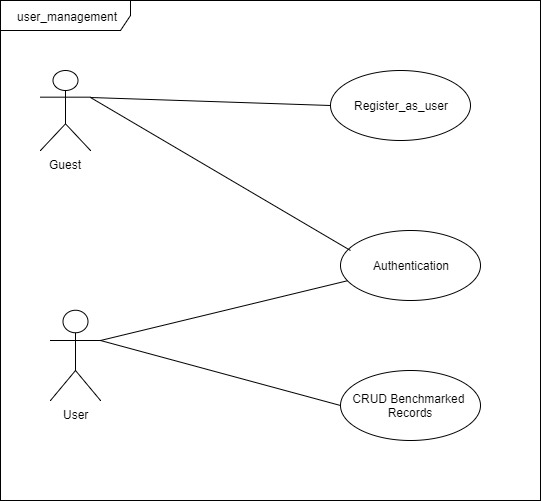
\includegraphics[width=15cm , height=10cm]{userDiagram.jpg}
        \newline 
        \textit{Figure 1} use case.
        \newline
        \newline No information is stored for the guest user. When accessing the service, the user
        assumes the guest role without being logged in. The guest user may use public
        services and my register or log in.
        When a user is registered, the fields shown in the domain model are stored for the
        user using a unique automatically assigned ID. The user provides all other fields. The
        password is stored in encrypted format. The user can access all the services provided by the service
        The register as user  use case is initiated by an end-user to create an account.\newline\newline
        A user will not be created if the email specified in the request to create a user is already
        associated with an existing user. This is done to ensure that if a user is already associated
        with the email address, the user is given access to his/her profile instead of creating a new
        user.\newline\newline
        Note that this use case will use the \textbf{getUser(userEmail)} service provided by the module to
        confirm if another user with that same email already exists in the system. A user should
        only be created if \textbf{getUser(userEmail)} throws the \textit{noSuchUser} exception.
        After the account has been created a notification will be sent to the user. The system have two types of users: Guest user and Registered user.
        
        \paragraph{\textbf{Precondition Table}}
        CU1 \textbf{getUserEmail(email)}
        \newline
        \newline
        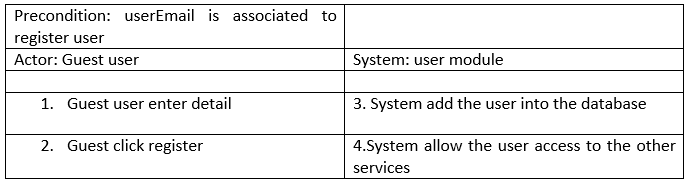
\includegraphics[width=12cm,height=3cm]{preUser.PNG}
        \newline 
        \textit{Figure 2} Precondition Table.

    
    
    \subsubsection{Display module}
        \paragraph{Scope}
        The display module constructs graphs, charts and tables to represent the benchmark results, and how different algorithms 
        compare against one another in terms of performance.
        
        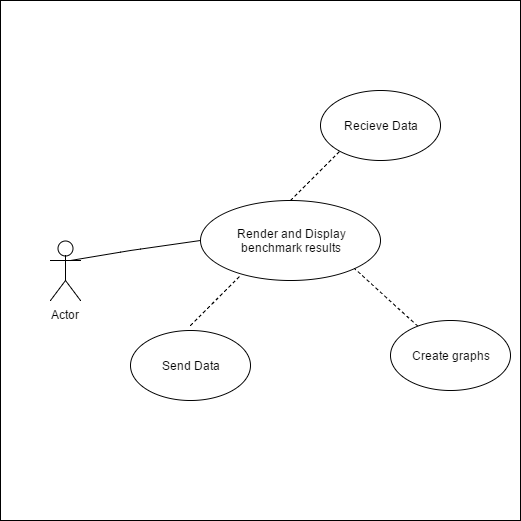
\includegraphics[width=7cm,height=7cm]{DisplayUseCase.png}
        \newline 
        \textit{Figure 3} use case.
        \newline
        \newline
        The display module concerns itself with rendering and displaying the results of benchmarks.
        The display module concerns itself primarily about creating graphs, charts and tables to represent the
        benchmarking results in a easily readable manner. 
        \newline
       
        \paragraph{\textbf{Technologies}}
        \newline
        When it comes to Display technologies, one in particular is of note.
         JFreeChart - A free 100% JAVA chart library that makes it easy for developers to display professional quality charts in their applications.
         JFreeChart's extensive feature set includes:
        	\item 1.A consistent and well-documented API, supporting a wide range of chart types;
        	\item 2.A flexible design that is easy to extend, and targets both server-side and client-side applications;
        	\item 3.Support for many output types, including Swing and JavaFX components, image files (including PNG and JPEG), and vector graphics file formats (including PDF, EPS and SVG);
        	\item 4.JFreeChart is open source or, more specifically, free software. It is distributed under the terms of the GNU Lesser General Public Licence (LGPL), which permits use in proprietary applications.\\
        	
    \subsubsection{Bench-marking and VM initializing Module}
        \paragraph{Scope}
        
        The module initializes and deploys VMs based on the request(s). On the VMs we will have a Java program that runs other programs, that is compile them, run them with the user specified data sets and then benchmark the program or algorithms. This module will initialize VMs on request and can initialize them concurrently within seconds.\\
        
        
        \paragraph{Technologies.}
        Osv - the open source operating system designed for the cloud. Built from the ground up for effortless deployment and management, with superior performance.\\
        
        Unikernels - specialized, single address space machine images constructed by using library operating systems(Osv in our case).We select, from a modular stack, the minimal set of libraries which correspond to the OS constructs required for our application to run.\\
   
    \subsubsection{Access Module}
        \paragraph{Scope}
        This module provides access to the system. The access channel will be web-front end, which refers to the ability of a user to use the system from a web browser(typically a well known one  such Chrome or Firefox). The access module also interacts with the other modules to integrate the system. 
        
        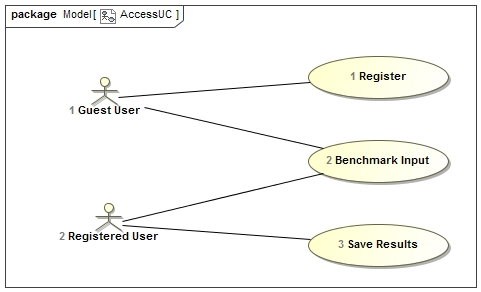
\includegraphics[width=15cm , height=10cm]{AccessUC.jpg}
        \newline 
        \textit{Figure 4} use case.
        \newline
        
    
   
	\subsection{External Interface Requirements}
		\begin{itemize}
			\item The user will communicate with the web interface, providing test algorithms and datasets as inputs.
			\item The Access module will receive the user inputs, validate correctness, and then send it to the benchmarking module. \newline
				Error checking will consist of ensuring the algorithms and datasets are compatible, as well as the code that is going to be executed is not harmful to the system (Eg. Infinite loops).
			\item The Benchmarking module will boot up a virtual machine to respond to this request, and send the user input through as parameters.
			\item The Access module will receive the results from the Benchmarking module, and then send it to the Display module.
			\item The Display module receives the results from the Access module and then draws visual representation on the Web Interface \newline
				If the user is a free or registered is determined at this stage and will determine how extensively drawn the output will be for the user.
			\item If the user is registered, then they will have the option to save their benchmarking data for later viewing, which will be performed by the Access module. \newline
				A MySQL database will be utilized for storing user data.
		\end{itemize}
	
%----------------------------------------

\subsection{Functional Requirements}
	\begin{EIREnum}
	    \item The system should enable create and manage user profiles
		\item The system should enable the user to upload source code
		\item The system should let the user choose the performance attribute to measure
		\item The system should run the algorithm
		\item The system should provide feed back to the user 
	\end{EIREnum}
	
\subsection{Performance Requirements}
    {\bf Efficiency}
        \begin{flushleft}
		Time Behaviour\newline 
		The benchmarking service should provide a response in at most 10sec, provided there are no delays pertaining to the internet connection.
	
		Resource Behaviour\newline
		The platform the system will be running on should use minimal resources (isolated machines) so that the side-effects that are not a concern
		of the specified benchmark is minimized.
		\end{flushleft}
	\newline
	{\bf Scalability}\newline
		The system should be able to handle a growing amount of work or be extended to accommodate growth. The total output should be able to increase 
		when resources are added.
    \newline
    \newline
	{\bf Reliabity}\newline
		The system should be able to compile and benchmark any algorithm written in java.
		The system should be available to any device that has a browser.
    \newline
    \newline
	{\bf Usability}\newline
		The system should be easy to use without any need for local configuration.



     
     
\end{document
